%\vspace{-2mm}
\section{Experiments, Results and Analysis} \label{sec:expt}
%\vspace{-2mm}
% \begin{figure*}[!thb]
% \centering
% \begin{subfigure}[t]{.35\textwidth}
%   \centering
%   \includegraphics[width=\linewidth]{./images/EventGNN.png}
%   \caption{Event-GNN}
%   \label{fig:ilsi-lfreq-ilb}
% \end{subfigure}%
% % \begin{subfigure}[t]{.24\textwidth}
% %   \centering
% %   \includegraphics[width=\linewidth]{./images/ParaGNN.png}
% %   \caption{Para-GNN}
% %   \label{fig:ilsi-lfreq-lf}
% % \end{subfigure}%
% \begin{subfigure}[t]{.60\textwidth}
%   \centering
%   \includegraphics[width=\linewidth]{./images/EnsembleGNN.png}
%   \caption{Ensemble}
%   \label{fig:echr-lfreq-ilb}
% \end{subfigure}%
% %\vspace{-4mm}
% \caption{Diagram of methods}
% %\vspace{-5mm}
% \label{fig:analysis-lfreq}
% \end{figure*}
%\subsection{Implementation Details} \label{sec:expt/implementation}
%\noindent\textbf
\begin{table*}[!thb]
    \centering
    \small
    \begin{tabular}{p{0.24\textwidth}p{0.22\textwidth}cccccc}
         \toprule
         \textbf{Method} & \textbf{Setting} & \multicolumn{3}{c}{\textbf{LSR}} & \multicolumn{3}{c}{\textbf{PCR}} \\
          & & \textbf{F1} & \textbf{MAP} & \textbf{MRR} & \textbf{F1} & \textbf{MAP} & \textbf{MRR} \\ \midrule 
        \multicolumn{8}{c}{\textbf{Lexical Methods}}\\ \midrule 
 
         \multirow{4}{0.24\textwidth}{Vanilla BM25 (full doc)} & 2-gram & 13.15& 14.54& 32.36& 24.89& 32.41& 47.21\\
          & 4-gram & 17.06& 19.13& 40.88& 30.54& 40.24& 54.65\\ 
          & 3-gram & 17.80& 19.39& 41.74& 32.21& 43.44& 57.52\\ 
          & 5-gram & 16.98& 17.88& 40.08& 33.29* & 43.98* & 58.55*\\ \midrule 

        \multirow{2}{0.24\textwidth}{Vanilla BM25 (para-wise)} & 2-gram, Max-All & 18.59& 21.82& 44.32& 27.87& 38.15& 52.32\\
        & 2-gram, Max-Sum & 14.66& 16.67& 35.84& 26.23& 35.26& 49.41\\ \midrule 
        

        
         \multirow{4}{0.24\textwidth}{Spacy events + BM25 (full doc)} & 2-gram & 12.65 & 14.48 & 32.08 & 24.91 & 33.02  & 48.22 \\
         & 3-gram & 10.67 & 11.93 & 28.12 & 28.31 & 37.22 & 52.70 \\
         & 4-gram & 10.18 & 10.47 & 26.40 & 28.28 & 35.30 & 50.98 \\
         & 5-gram & 9.78 & 9.52 & 25.28 & 26.99 & 33.71 & 50.22 \\ \midrule 
         
         \multirow{4}{0.24\textwidth}{LLM events + BM25 (full doc)} & 2-gram & 13.08& 14.47& 32.49& 24.55& 31.78& 46.10\\
         & 3-gram & 16.84& 18.76& 40.60& 29.47& 38.59& 52.97\\
         & 4-gram & 17.45& 18.92& 41.34& 32.61& 42.99& 57.39\\
         & 5-gram & 16.41& 17.35& 39.33& 33.29& 43.43& 58.14\\ \midrule 
         


         \multicolumn{8}{c}{\textbf{Semantic Methods}}\\ \midrule 

         
         \multirow{3}{0.24\textwidth}{SAILER (full doc)} & inference  & 7.15& 9.31& 19.40& 9.94& 13.90&20.49\\
         & fine-tune separately  & 21.69 & 28.62& 45.73&  12.64& 17.93&  25.85\\ 
         & fine-tune multi-task & 20.45& 25.36& 41.44& 11.88& 17.52& 24.85\\ \midrule 
         
         \multirow{2}{0.24\textwidth}{SAILER (para-wise)} & inference, Max-All & 13.11 & 14.70 & 31.49 & 19.37 & 25.71 & 38.84  \\
        & inference, Max-Sum & 5.42 & 6.57 & 16.06 & 11.16 & 16.42 & 24.67 \\ \midrule 
        \multirow{2}{0.24\textwidth}{SAILER (summaries)} & inference & 5.48& 7.66& 16.86& 10.21& 14.80& 22.82\\
        & fine-tune separately & 23.49& 31.42& 50.25& 15.00& 20.43& 27.72\\ \midrule 
        
         \multirow{2}{0.24\textwidth}{Event-GNN (full doc)} & fine-tune separately & 28.67 & 38.69 & 58.39&  12.08& 15.91&  22.18\\ 
         & fine-tune multi-task & 18.43& 24.11& 43.23& 11.74& 15.59& 22.56\\ \midrule 
         \multirow{2}{0.24\textwidth}{Para-GNN (full doc)} & fine-tune separately & 20.72& 28.54& 46.06&  24.54  & 33.07& 45.01\\ 
         & fine-tune multi-task & 23.74& 29.79& 49.84&  24.67& 32.88& 44.17\\ \midrule 
         
        
         \multirow{2}{0.24\textwidth}{Para-GNN (summaries)} & fine-tune separately & 32.85* & 44.03* & 62.51&   22.60& 29.49& 39.22\\ 
         & fine-tune multi-task & 31.81& 43.17& 64.08* & 22.69& 29.25& 39.19\\ \midrule 
         
         \multicolumn{8}{c}{\textbf{Ensemble Methods}}\\ \midrule 
         \multirow{3}{0.24\textwidth}{Event-GNN + BM25} & Grid Search & 33.87 & 45.17 & 67.26 & 34.45 & 43.32 & 58.76 \\
         & Dyn. $\alpha$, fine-tune separately & 30.29 & 40.97 & 61.51 & 35.60 & 45.86 & 60.89 \\
         & Dyn. $\alpha$, fine-tune multi-task & 25.62 & 31.97 & 57.01 & 35.63 & 45.18 & 60.51 \\ \midrule 
          \multirow{3}{0.24\textwidth}{Para-GNN (full doc) + BM25} & Grid Search & 28.10 & 36.14 & 59.57 & 36.93 & 48.62 & 62.83 \\
          & Dyn. $\alpha$, fine-tune separately & 27.05 & 35.20 & 59.67 & 36.91 & 48.53 & 62.61 \\
          & Dyn. $\alpha$, fine-tune multi-task & 27.01 & 33.57 & 59.00 & 36.57 & 48.18 & 62.14 \\ \midrule 
          \multirow{4}{0.24\textwidth}{Para-GNN (summaries) + BM25} & Grid Search& 36.17 & 48.64 & 70.49 & 36.35 & 48.27 & 61.76 \\
          & Dyn. $\alpha$, fine-tune separately & 38.09&  50.31&  70.54& 37.46 &  48.28&  61.98\\
          & Dyn. $\alpha$, fine-tune multi-task & 35.91 &  46.95&  68.57& 37.82 &  49.54&  63.61\\
          & Dyn. $\alpha$, fine-tune transfer learning & \underline{39.44}&  \underline{52.13}&  \underline{73.77}& \underline{38.77}&  \underline{50.21}&  \underline{63.81}\\ \midrule 
          \multicolumn{8}{c}{\textbf{LLM Re-ranking}}\\ \midrule 
          \multirow{2}{0.24\textwidth}{GPT-4.1} & First-stage prompt & 45.29& 59.73& 81.02& 41.54& 52.80& 67.16\\
          & Second-stage prompt & \textbf{46.11}& \textbf{61.06}& \textbf{81.55}& \textbf{43.31}& \textbf{54.43}& \textbf{68.88}\\
          \bottomrule
         % \hline
    \end{tabular}
    \vspace{-2mm}
    \caption{Results (\%) of Statute retrieval and Precedent retrieval. Metrics are macro-F1@k, MAP and MRR. Best value for each metric in boldface. Best values before re-ranking underlined, and best values for individual methods (not ensemble methods) marked with asterisk(*). We also calculate statistical significance of results  (App.~\ref{app:sigtest}).}
    \label{tab:results}
    \vspace{-5mm}
\end{table*}
%\vspace{-2mm}
%\subsection{Results} \label{sec:expt/results}
%\vspace{-2mm}
% \old{The results of all methods are presented in Table~\ref{tab:results} in terms of standard evaluation metrics macro-F1@k, MAP and MRR (details in App. \ref{app:expt/datasets}). We observe a stark difference in the performance of different methods for statutes and precedents.  
% Methods based on BM25, which focus on lexical matches and hence can capture legal phrases or keywords, are very effective for precedent retrieval.
% Whereas, fine-tuned transformer models are able to perform better for statute retrieval than unsupervised lexical methods.
% %, where all the fine-tuning approaches significantly outperform the unsupervised approaches. 
% The language used in statute descriptions is more formal than that used in case documents, and thus direct keyword matching can be difficult. This could explain why supervised fine-tuning is performing the best. 
% %We also observe that tuning statutes and precedents jointly in a multi-task learning setup does not perform as well as the setup where they are tuned separately (more on this in Section~\ref{sec:expt/results/statprec}).
% Also, we observe that summarization leads to an improvement in performance only for statutes, but not precedents (compared to taking the full documents as input).}

\noindent The results of all experiments are presented in Table~\ref{tab:results} in terms of standard evaluation metrics macro-F1@$k$, MAP and MRR (details in App.~\ref{app:expt/datasets}, hyper-parameters in App.~\ref{app:implementation}). 

\vspace{1mm}
\noindent\underline{\textbf{Performance over LSR:}} 
% We observe that the lexical approaches perform rather poorly over LSR, possibly due to the abstract and technical language used for statutes. 
% While the para-wise variant of BM25 improves results, these are quite poor compared to the performance of semantic, fine-tuned methods. 
% Among these, utilizing the LLM retrieval-focussed summaries with the Para-GNN architecture proves the most effective (32.85\% F1), while summaries over full document input are helpful for other methods like SAILER as well. 
Lexical methods perform poorly on statute retrieval, likely due to the abstract and technical phrasing of statutes. Even the best lexical variant (BM25, para-wise Max-All) achieves only 18.59\% F1. In contrast, fine-tuned semantic models show large gains, with Para-GNN (summaries) reaching 32.85\% F1---a relative improvement of nearly 77\%. This highlights the need for deeper contextual modeling. Summaries also help other semantic models such as SAILER, though the gains are smaller. 

\vspace{1mm}
\noindent\underline{\textbf{Performance over PCR:}} 
% In the case of PCR, we observe the reverse trends as compared to LSR. The semantic, fine-tuning based methods underperform as compared to lexical methods like BM25. Among these, Para-GNN again performs the best, although there is a slight drop in performance on using summaries over full documents. We suspect that PCR depends on exact lexical matches over short contextual windows for both queries and precedents, and thus using summaries can lead to information loss. In a broader sense, the same factor, coupled with the fact that both queries and precedents are long documents makes the task non-conducive for semantic fine-tuning methods.
In contrast to LSR, lexical methods clearly dominate PCR. The best lexical model (BM25, 5-gram) achieves 33.29\% F1, whereas the strongest semantic model (Para-GNN, full doc, fine-tuned) reaches only 24.67\% F1, a relative drop of about 26\%. Moreover, summaries further reduce performance, suggesting that essential lexical cues are lost during compression. These results indicate that PCR depends heavily on exact lexical matches within short contextual windows, and the long, detailed nature of queries and precedents makes semantic fine-tuning less effective. 



\begin{figure*}
\begin{subfigure}[t]{.47\linewidth}
  \centering
  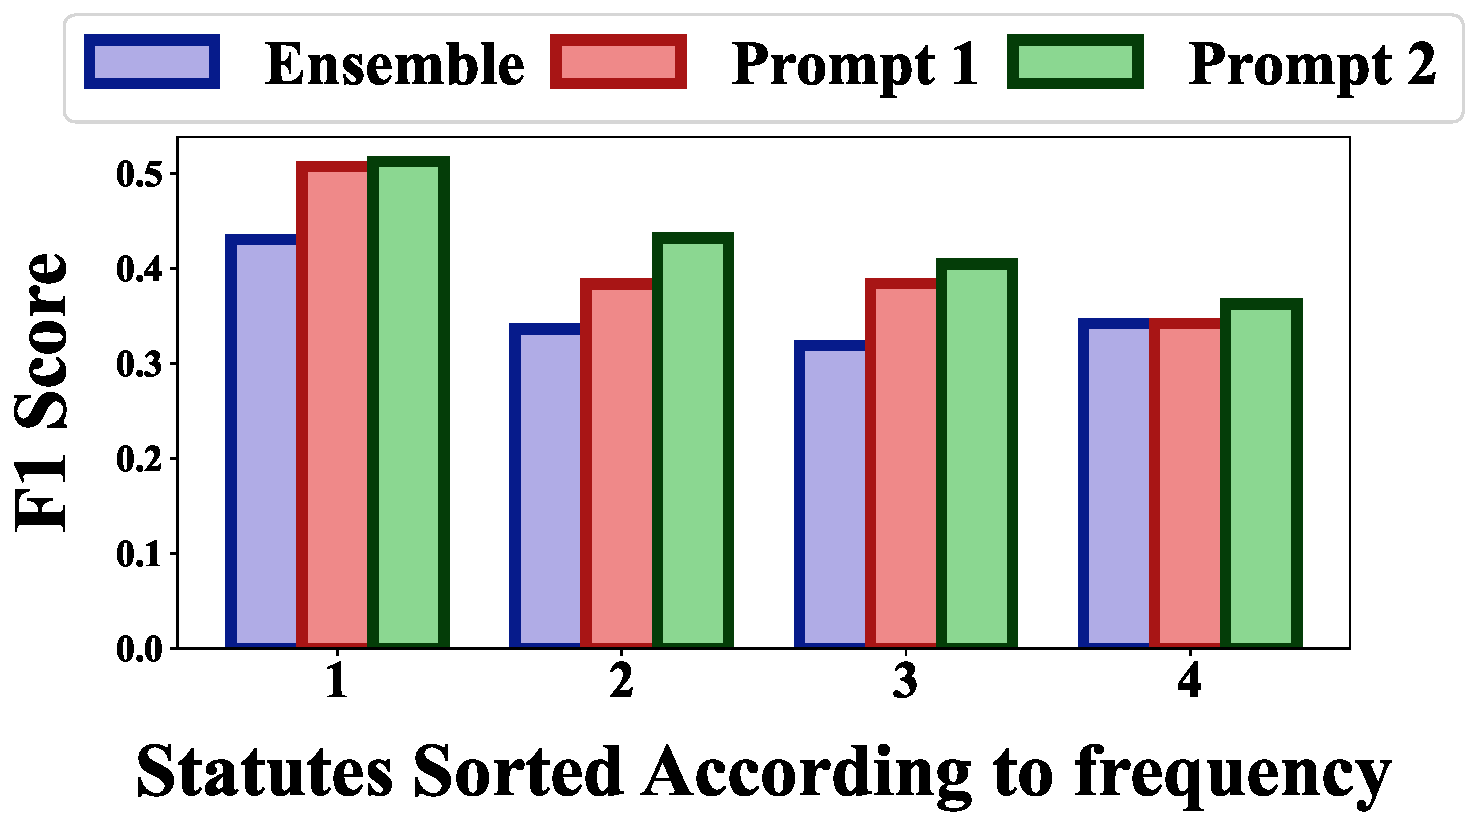
\includegraphics[width=\linewidth]{./images/llm-freq-lsr.pdf}
  \caption{LSR F1 vs. frequency}
  \label{fig:llm-freq-lsr}
\end{subfigure}%
\hfill
\begin{subfigure}[t]{.47\linewidth}
  \centering
  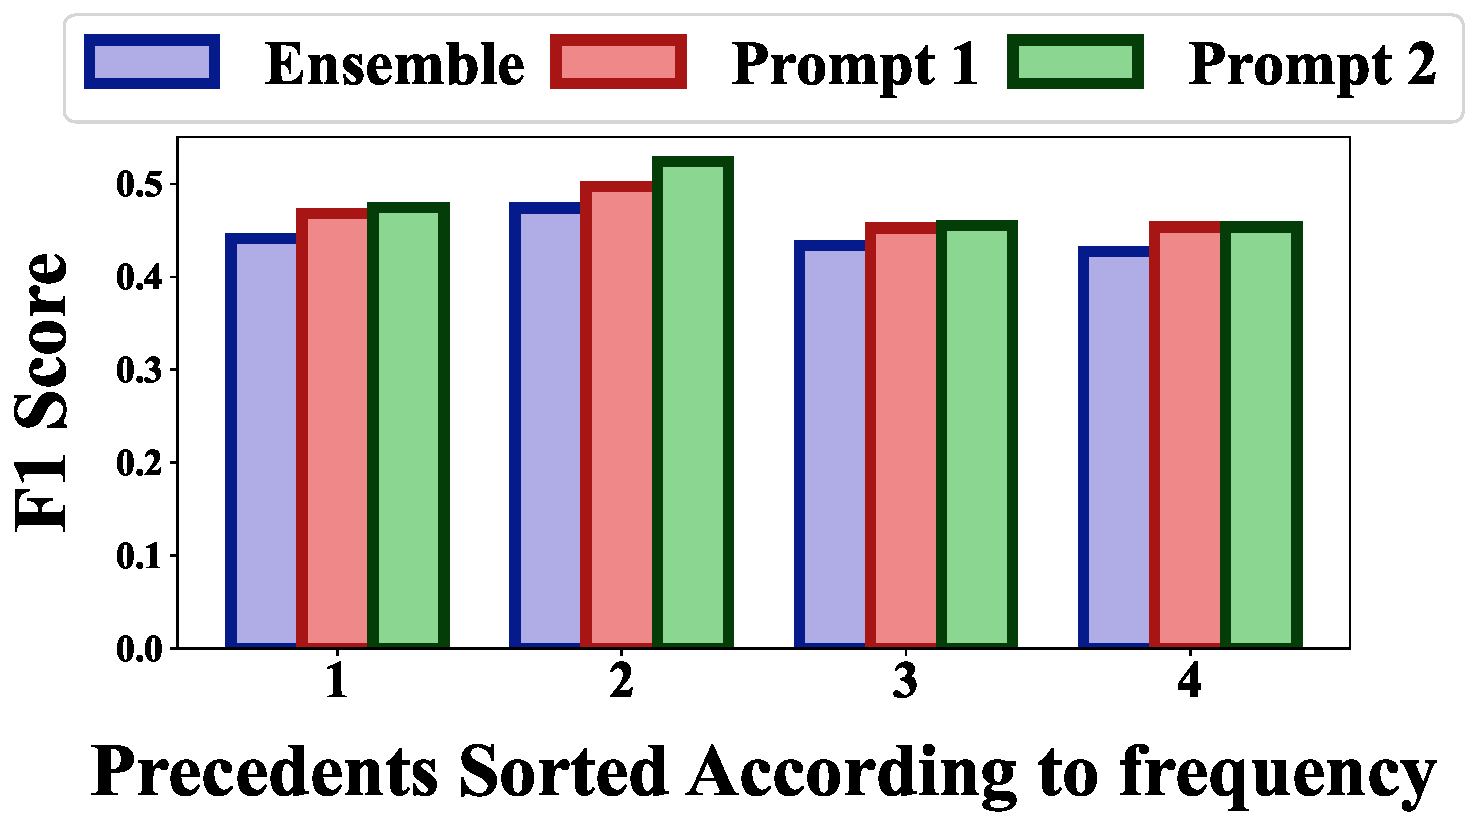
\includegraphics[width=\linewidth]{./images/llm-freq-pcr.pdf}
  \caption{PCR F1 vs. frequency}
  \label{fig:llm-freq-pcr}
\end{subfigure}%
\vspace{-2mm}
\caption{Performance in terms of F1(\%) compared to frequency of candidates. On the X-axis, the candidates are sorted from left to right according to frequency and divided into groups (most frequent group-1, most rare group-4).} 
\label{fig:llm-freq}
\vspace{-5mm}
\end{figure*}

\vspace{1mm}
\noindent\underline{\textbf{Results of Ensemble Models:}}
% The ensemble approaches achieve improvements for both statutes and precedents, compared to both the individual lexical and semantic methods. This is true for all three variants of the semantic method (Event-GNN, Para-GNN with full docs and summaries). Although the dynamic $\alpha$ method slightly underperforms compared to grid search for Event-GNN + BM25 and Para-GNN (full doc) + BM25, there are clear gains over grid search in the case of Para-GNN (summaries) + BM25 for both LSR (38.09\% vs. 36.17\% F1) and PCR (37.46\% vs. 36.35\% F1). 
Combining lexical and semantic features consistently improves performance for both LSR and PCR compared to individual methods. This trend holds across Event-GNN, Para-GNN (full doc), and Para-GNN (summaries). While the dynamic $\alpha$ method slightly underperforms grid search for Event-GNN + BM25 and Para-GNN (full doc) + BM25, it yields clear gains for Para-GNN (summaries) + BM25. F1 improves from 36.17\% to 38.09\% for LSR, and from 36.35\% to 37.46\% for PCR. These findings show that \textit{ensemble models effectively combine the complementary strengths of lexical and semantic approaches.}


% \noindent We also investigated combining above approaches for LSR and PCR together. %The promising results mentioned before are for the separate fine-tuning setup, and thus we investigate the performance of the same approach combining LSR and PCR together. 
% The first variant, joint multi-task tuning over both tasks, leads to small improvement in PCR but a huge drop in performance for LSR (from 38.09\% to 35.91\%). Results also show that joint fine-tuning does not perform as well as separate fine-tuning, including the other ensemble variants and the pure semantic methods themselves. The \textit{difference in nature of the candidates for the two tasks} creates difficulty for any model to learn the relationships between a query, and its cited statute and precedent candidates simultaneously.
% However, when we conduct transfer learning (LSR $\rightarrow$ PCR or PCR $\rightarrow$ LSR) on the Para-GNN (summaries) + BM25 method, we obtain the best results at the ensemble stage (39.44\% F1 for LSR, 38.77\% F1 for PCR). This shows that a model trained on one task can be utilized to further improve the other task, and points towards an inherent relationship between the two tasks which can be exploited effectively. However, \textit{a sequential setup like transfer learning is more conducive for better performance on both tasks as compared to joint multi-task learning}. %, which is reported in App.~\ref{app:gridsearch}.}

\noindent Joint multi-task fine-tuning does \textit{not} outperform separate fine-tuning. PCR gains are marginal, while LSR performance drops (38.09\% $\rightarrow$ 35.91\% F1). This is possibly due to \textit{task interference}, a well-documented issue in multi-task learning where conflicting gradient signals across even related tasks degrade performance~\citep{mueller-etal-2022-text2text,ni-etal-2023-multitask}. 
In our case, LSR needs robust semantic features, whereas PCR depends more on lexical overlaps. These divergent retrieval signals create interference under joint optimization, making it difficult for a shared model to specialize in both.  
In contrast, transfer learning (LSR $\rightarrow$ PCR or PCR $\rightarrow$ LSR) decouples representation learning from task specialization. Pre-training on one task provides a useful legal inductive bias, while subsequent fine-tuning adapts to the target task without interference. This gives the best ensemble results, with 39.44\% F1 (LSR) and 38.77\% F1 (PCR), representing +20\% and +16\% improvements over the strongest standalone models (Para-GNN with summaries for LSR, BM25 5-gram for PCR).  
Thus, LSR and PCR tasks \textit{despite being interdependent, suffer from task interference during joint training; using sequential transfer avoids this}, improving over both independent and joint training.

\vspace{1mm}
\noindent\underline{\textbf{Re-ranking with LLMs:}}
% We proceeded with the best ensemble method, and use the top 20 statutes and top 10 precedents for re-ranking with \texttt{gpt-4.1} (\url{https://platform.openai.com/docs/models/gpt-4.1}). In the first prompting stage, LSR and PCR re-ranking are performed completely independently using the outputs of the ensemble model. 
% In this stage itself, we obtain massive gains for the LLM over the ensemble model, both in the case of LSR (45.29\% vs. 39.44\% F1) and PCR (41.54\% vs. 38.77\% F1). The LLM is able to utilize its superior legal language understanding capabilities, to improve upon both tasks.
% In the second stage, we utilize the outputs from the first stage of one task as additional inputs for the second stage of the other task. In both these settings, i.e., $\textrm{LSR}_1 \rightarrow \textrm{PCR}_2$ and  $\textrm{PCR}_1 \rightarrow \textrm{LSR}_2$, the final output is better in terms of performance than the first-stage outputs, achieving the best results for both LSR (39.44\% F1) and PCR (38.77\% F1) among all experiments.
% The LLM is able to utilize its powerful legal reasoning capabilities to exploit the relationship between statutes and precedents via the second stage prompt.
% \textit{This experiment establishes our intuition that inherently related tasks of LSR and PCR can be used to improve each other}.
We build on the best ensemble model by re-ranking the top-20 statutes and top-10 precedents using \texttt{gpt-4.1} (\url{https://platform.openai.com/docs/models/gpt-4.1}). In the first stage, LSR and PCR are re-ranked independently. The LLM delivers substantial improvements over the ensemble baseline, raising F1 from 39.44\% to 45.29\% for LSR and from 38.77\% to 41.54\% for PCR highlighting stronger legal language understanding.  
In the second stage, outputs from one task are provided as additional inputs to the other (i.e., $\textrm{LSR}_1 \rightarrow \textrm{PCR}_2$ and $\textrm{PCR}_1 \rightarrow \textrm{LSR}_2$). This cross-task conditioning further boosts performance, yielding 46.11\% F1 for LSR (+1.8\% over stage~1) and 43.31\% F1 for PCR (+4.3\% over stage~1). These additional gains directly reflect the interdependence between statutes and precedents, as improvements in one task propagate to the other.
Thus, \textit{LLM re-ranking achieves state-of-the-art results for both tasks, reaffirming the intuition that improvements in one task enhance the other.}



% \old{Utilizing LLMs to predict the relevance for the top-$K$ candidates based on the ranked lists produced by best method described in the last paragraph, leads to massive improvements in performance for both LSR (44.20\% vs. 39.43\% F1) and PCR (43.01\% vs. 41.53\%). GPT-4.1 utilizes its superior language understanding capabilities and legal knowledge acquired during pre-training to identify the relevant candidates, thereby ranking them higher in the re-ranked list. In the pipeline prompting setup, for LSR, including extra statutes (apart from top-$K$) that are cited by relevant precedents of the same query, gives the LLM an oppurtunity to look at more candidates, thereby improving the re-ranking performance to 45.19\% F1 compared to baseline re-ranking of 44.20\%. For PCR, providing the relevant statutes of the query and precedent along with the texts allows the LLM to utilize its legal reasoning capabilities to better determine relevance, improving the final score to 43.01\% F1 vs. 41.53\% for baseline re-ranking. This shows us that LLMs can effectively utilize the knowledge gained from solving either task, to then improve the performance over the other task.}



\begin{table*}[!thb]
    \centering
    \small
    \begin{tabular}{p{0.28\textwidth}p{0.22\textwidth}cccc}
         \toprule
         \textbf{Method} & \textbf{Setting} & \multicolumn{2}{c}{\textbf{LSR}} & \multicolumn{2}{c}{\textbf{PCR}} \\
          & & \textbf{Cited} & \textbf{Cited + Annot.} & \textbf{Cited} & \textbf{Cited + Annot.} \\ \midrule 
        
         
         \multicolumn{6}{c}{\textbf{Ensemble Methods}}\\ \midrule 
          \multirow{3}{*}{Para-GNN (summaries) + BM25} & Dyn. $\alpha$, ft. separately & \underline{43.27} & \underline{51.78} & 42.19 & \underline{47.02} \\
          & Dyn. $\alpha$, ft. multi-task & 38.90&  46.90&  \underline{42.55}& 45.21\\
          & Dyn. $\alpha$, ft. transfer learning & 43.22&  51.22&  42.41& 45.11\\ \midrule 
          \multicolumn{6}{c}{\textbf{LLM Re-ranking}}\\ \midrule 
          GPT-4.1 & First-stage prompt & 47.06& 56.72& 45.33& 46.88\\
          GPT-4.1 & Second-stage prompt & \textbf{47.77}& \textbf{57.72}& \textbf{46.93}& \textbf{47.63}\\
          \bottomrule
         %\hline
         % Ensemble (RR-GNN + BM25) & Grid Search & 28.10& 36.14& 59.57& 36.93& 48.62& 62.83\\ 
         % Ensemble (RR-GNN + BM25) & Dynamic Alpha & 27.05& 35.20& 59.67& 36.91& 48.53& 62.61\\
         % Ensemble (Event-GNN + BM25) & Grid Search & 33.87 & 45.17 & 67.26 & 34.45& 43.32& 58.76\\ 
         % \hline
    \end{tabular}
    \vspace{-2mm}
    \caption{Results (\%) of Statute retrieval and Precedent retrieval in terms of macro-F1@k, considering only Cited candidates vs. union of Cited and Annotated candidates as the gold-standard. Best value for each metric in boldface and best values before re-ranking are underlined.}
    \label{tab:human-results}
    \vspace{-5mm}
\end{table*}



% \noindent\textbf{Effect of candidate frequencies on LLM Re-ranking:}\label{sec:expt/freq}
% To further analyze the re-ranking results, we study the examine the performance of different methods/stages of our entire pipeline, with respect to the frequency of the candidate. Specifically, we compare between the Ensemble of Para-GNN (summaries) + BM25, dyn. $\alpha$ fine-tuning with transfer learning, and the two LLM prompting stages involving GPT-4.1. For both tasks, we take all candidates, sort them in descending order of frequency and divide into 4 groups numbered 1-4 (Group-1 having the most frequent candidates, Group-4 having the most rare), and plot the macro-F1 scores for each group in Fig.~\ref{fig:llm-freq}. In the case of LSR (Fig.~\ref{fig:llm-freq-lsr}) we observe that the first-stage LLM prompting provides significant improvement across all groups except the rarest (Group-4), demonstrating the superior performance of the LLM across a wide range of statute frequencies. The second-stage prompting increases the re-ranking range of the LLM by providing more statutes (cited by first-stage re-ranked precedents), which proves to be beneficial particularly for Group-2 and Group-4 (rarest statutes).
% Fig.~\ref{fig:llm-freq-pcr} shows the plot for PCR after following the same steps as LSR. Similar to LSR, PCR performance also increases across all groups using first-stage prompting. However, unlike LSR, the second-stage prompting provides minimal improvement over the rare precedents (Groups-3,4), with the most improvement observed for Group-2 (more details in App. \ref{app:freqanalysis} and \ref{app:lenanalysis}).
\noindent\textbf{Effect of candidate frequency on LLM re-ranking:}   
To further analyze re-ranking behavior, we examine performance with respect to candidate frequency. All candidates are sorted in descending order of frequency and divided into four groups (Group-1 most frequent, Group-4 rarest), and macro-F1 is computed for each (Fig.~\ref{fig:llm-freq}).  

\noindent For \textbf{LSR} (Fig.~\ref{fig:llm-freq-lsr}), first-stage prompting substantially improves over the ensemble across Groups~1--3, demonstrating stronger performance on frequent and moderately frequent statutes. Stage-2 prompting further expands the re-ranking range by incorporating statutes cited by re-ranked precedents, which is particularly beneficial for Group-2 and Group-4, showing that cross-task signals help cover rarer statutes more effectively.  

\noindent For \textbf{PCR} (Fig.~\ref{fig:llm-freq-pcr}), first-stage prompting again provides consistent improvements across all groups. Stage-2 prompting gives the largest additional gains for Group-2, while maintaining stable performance for rarer precedents (Groups~3 and~4). This indicates that cross-task conditioning reinforces retrieval for moderately frequent precedents, while preserving robustness on the long tail.  

\noindent LLM prompting is effective across frequency ranges, with Stage-2 re-ranking particularly valuable for mitigating weaknesses in mid- and low-frequency candidates, thereby reinforcing the cross-task dependency between LSR and PCR (more details in App. \ref{app:prompts}).

\vspace{1mm}
\noindent\underline{\textbf{Key Findings:}} 
% We observed that \textit{an ensemble of lexical and semantic methods usually perform the best for both LSR and PCR}, with the Ensemble Para-GNN + BM25 dynamic $\alpha$ method (summaries as input) perform the best among all first stage retrievers. This model was fine-tuned in a transfer learning fashion (LSR $\rightarrow$ PCR as well as PCR $\rightarrow$ LSR). This performance can be further boosted by using a two-stage LLM-based re-ranking technique, where the second stage of one task is dependent on the first stage output of the other task. Both for the retrieval and re-ranking phases, a pipeline approach that utilizes the outputs/knowledge of solving LSR to then eventually perform PCR proves to be the most effective (and vice-versa as well). To test  generalizability of our methods, we also experimented with COLIEE PCR dataset on Canadian cases, we observed similar trends. Due to space constraints we provide details in App. \ref{sec:coliee}.
Our experiments yield two primary findings. First, \textit{ensembles of lexical and semantic models consistently outperform individual approaches}, with Para-GNN (summaries) + BM25 under dynamic $\alpha$ fine-tuning giving the strongest first-stage retrieval results. Transfer learning between LSR and PCR also proves effective, although multi-task training does not provide comparable gains. Second, \textit{LLM-based re-ranking achieves the best overall performance}, with Stage-2 prompting---where outputs of one task condition the other---providing additional gains and \textbf{\textit{directly exploiting the LSR--PCR dependency}}. Taken together, these results establish that LSR and PCR, though traditionally studied in isolation, are \textbf{\textit{inherently connected tasks that can be leveraged jointly for stronger legal retrieval}}. For completeness, App.~\ref{sec:coliee} also reports experiments on the COLIEE dataset.


